\chapter{Software process models}
\emph{Software process models} define how to organize activities (e.g.,\@ requirement, design, \dots) and techniques that can be used to perform them (e.g.,\@ UML modelling, programming languages, testing, \dots).

\section{Phases and activities}
ISO/IEC 12207 defines how to identify processes, entities responsible of processes and products of each process. As shown in figure~\ref{img:iso_iec_12207}, the standard defines:
\begin{itemize}
\item Primary processes:
\begin{itemize}
\item Acquisition;
\item Supply;
\item Development;
\item Operation;
\item Maintenance.
\end{itemize}
\item Supporting processes:
\begin{itemize}
\item Documentation of product;
\item Configuration management;
\item Quality assurance:
\begin{itemize}
\item Verification \& Validation;
\item Reviews with customers;
\item Internal audits;
\item Problem analysis and resolution.
\end{itemize}
\end{itemize}
\item Organizational processes:
\begin{itemize}
\item Project management;
\item Infrastructure management:
\begin{itemize}
\item Facilities, networks, tools.
\end{itemize}
\item Process monitoring and improvement;
\item Training.
\end{itemize}
\end{itemize}

ISO 12207 only lists activities, independently of process model, technology, application domain and documentation.

\section{Process models}
A \emph{process model} defines how to organize activities, identifying roles, responsibilities, temporal constraints between activities satisfying constrains as laws or standards.

\subsection{Models}
Main constraints in defining a process model are:
\begin{itemize}
\item New development vs maintenance;
\item Compliance to standard or laws, related to criticality;
\item Size of end product, related with effort, calendar duration, size of staff involved, number and geographical distribution of teams.
\end{itemize}
Main operations in defining a process model are:
\begin{itemize}
\item Sequential vs parallel activities;
\item Iterations (a long one vs many short ones);
\item Emphasis or not on documents.
\end{itemize}

\paragraph{Build and fix}
\emph{Build and fix} model does not require any requirement, design or their validation. In fact, it is suitable only for solo programming and does not scale up for larger projects.

\paragraph{Waterfall}
\emph{Waterfall} [Royce 1970] is a document driven model which enforces sequential activities, each one producing a document used by the next one when the previous terminates.

It tends to use one long iteration, which is never feasible in practice because a change to a document implies re-doing all activities depending on it. Therefore, changes are long and expensive, leading to a lack of flexibility and tension to avoid changes.

Waterfall approach is suitable for large projects, distributed teams or contractors and mostly new developments where compliance is ensured by document. 

\begin{figure}[hbtp]
\centering
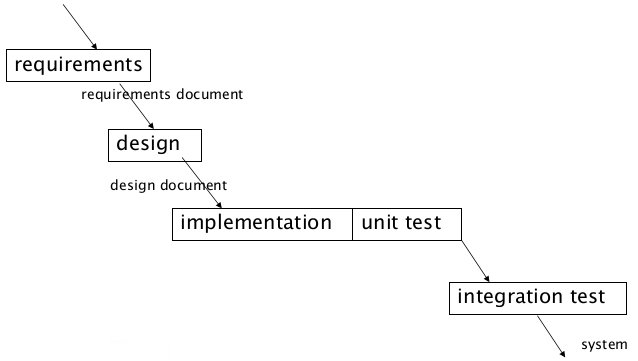
\includegraphics[scale=0.3]{images/waterfall_model.png}
\caption{Waterfall model}
\end{figure}

\emph{V model} is similar to waterfall, with emphasis on verification and validation activities. In fact, acceptance tests are written with requirements and unit or integration tests are written during design.

\paragraph{V model}
\begin{figure}[hbtp]
\centering
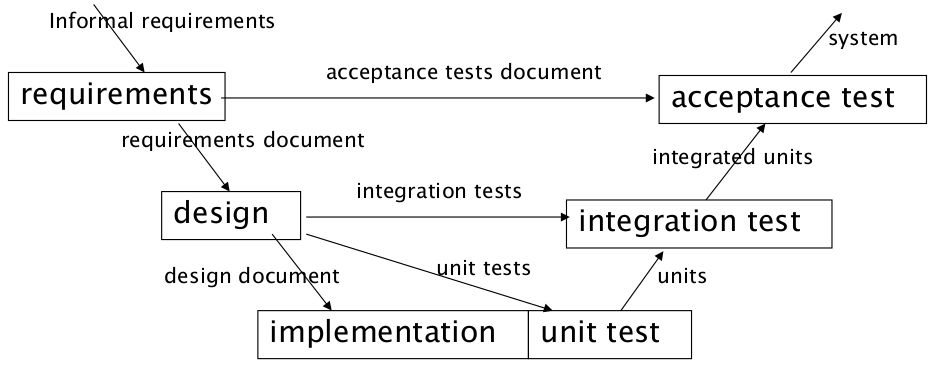
\includegraphics[scale=0.3]{images/v_model.png}
\caption{V model}
\end{figure}

\begin{figure}[hbtp]
\centering
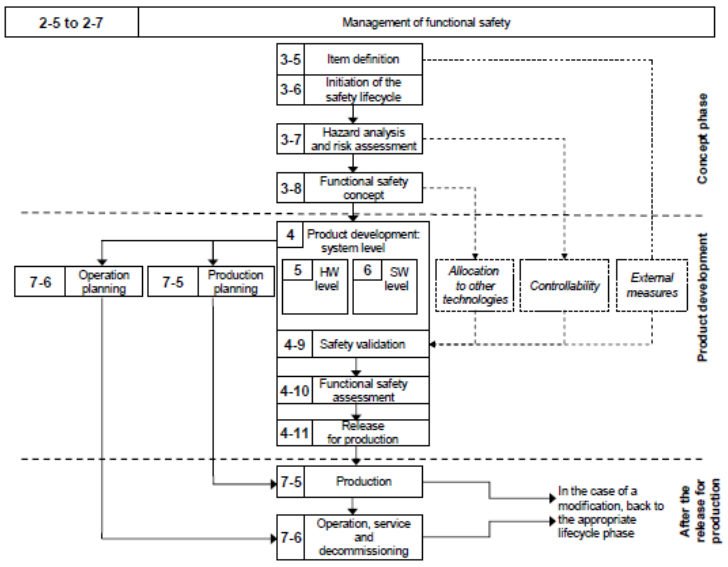
\includegraphics[scale=0.3]{images/safety_lifecycle.png}
\caption{Safety lifecycle}
\end{figure}

ISO 26262 and IEC 61508 are examples of V models. The first one is used in development of road vehicles requiring functional safety, which is an adaption of IEC 61508 used in safety industrial processes.

\begin{figure}[hbtp]
\centering
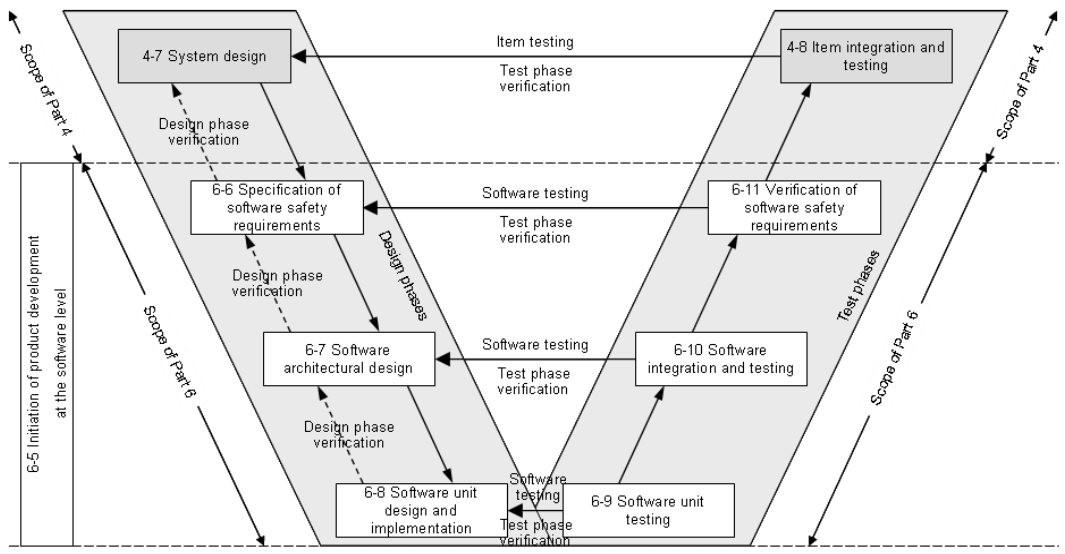
\includegraphics[scale=0.3]{images/software_lifecycle.png}
\caption{Software lifecycle}
\end{figure}

\paragraph{Prototyping}
\emph{Prototyping} consists of first building a quick and dirty prototype to validate and analyze requirements, then it is possible to proceed in a waterfall strategy. A software prototype is a product with less functions, possibly built in different platform, for instance a final embedded system produced in C can have a prototype written in Java or MATLAB emulated on a PC. The idea can be applied to other parts of a project, e.g.,\@ GUI prototyping, design prototyping, performance.

\begin{figure}[hbtp]
\centering
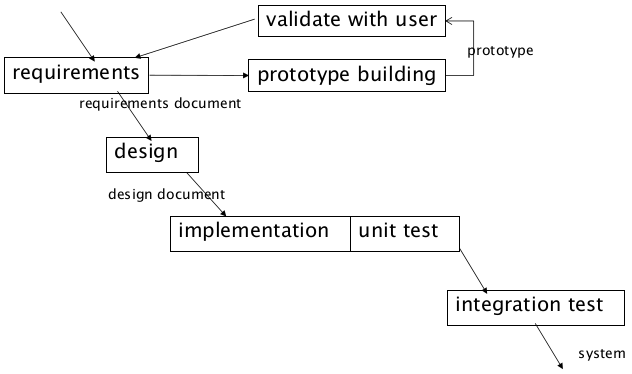
\includegraphics[scale=0.3]{images/prototyping_model.png}
\caption{Prototyping and waterfall model}
\end{figure}

In this way, it is possible to clarify requirements but this technique requires specific skills to build prototype, e.g.,\@ prototyping language and it would introduce business pressures to keep prototype, if successful, as final deliverable.

\paragraph{Incremental}
In waterfall, integration activity produces the complete system, that is delivered to costumer in one single shot. \emph{Incremental} model is the same as waterfall, but integration is split in such a way that every loop in integration produces a part of the system, therefore the system is delivered in several increments.

\begin{figure}[hbtp]
\centering
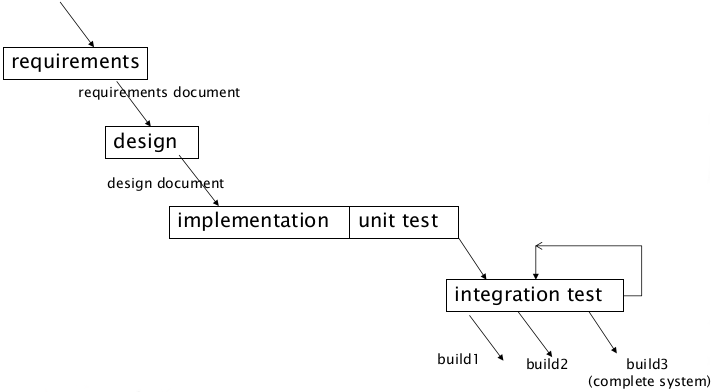
\includegraphics[scale=0.3]{images/incremental_model.png}
\caption{Incremental model}
\end{figure}

In this way it is possible to have an earlier feedback from user/customer and increments depending on external components can be delayed.

\paragraph{RUP}
\emph{Ration Unified Process} has been proposed in 1999. Activities are performed in parallel in one long iteration with sub-iterations exploiting a partial emphasis on documents. Iterations and deliveries (official releases) are planned and establish a point in time when everyone makes documents and code coherent and consistent with the others. In fact, this approach gives more flexibility and speed, but divergences are possible and must be limited.

\begin{figure}[hbtp]
\centering
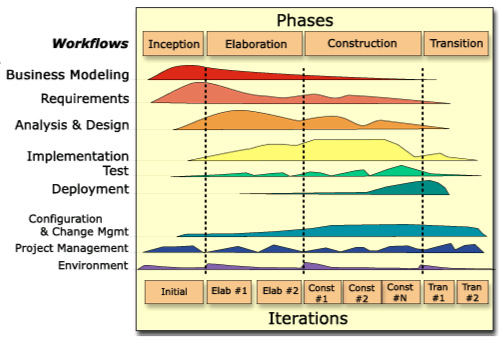
\includegraphics[scale=0.4]{images/rup_model.png}
\caption{RUP model}
\end{figure}

\begin{description}
\item [Inception] Feasibility study, risk analysis, essential requirements and possibly prototyping.
\item [Elaboration] Requirement analysis, architecture definition and project plan.
\item [Construction] Analysis, design, implementation and testing.
\item [Transition] Beta testing, performance tuning, documentation, training and packaging for shipment.
\end{description}
This approach is suitable for mostly new developments of possibly large projects, carried out by distributed teams, which require just partial compliance.

\paragraph{Reuse}
Most projects reuse components which can be open or closed source, free or not free. Therefore, availability is immediate, often with higher quality and lower cost but it leads to some issues like ownership of source, trade offs and loss of control on evolution.

It is needed to consider what is (un)available from components and change requirements accordingly. Components must be selected and evaluated, considering constraints and issues from components and adapt design consequently.

\begin{itemize}
\item Search and analysis of components;
\item Adaptation of requirements;
\item Design;
\item Implementation.
\end{itemize}

\subsection{Agile}
\emph{Agile} is a methodology where activities are performed in parallel in many short iterations without any emphasis on documents, i.e.,\@ just code and test cases, written as code.

This approach is suitable for both new developments on small projects and maintenance activities, carried out by co-located teams, without any compliance because no document is produced.

\paragraph{Agilemanifesto.org}
\begin{itemize}
\item Individuals and interactions over processes and tools;
\item Working software over comprehensive documentation;
\item Customer collaboration over contract negotiation;
\item Responding to change over following a plan.
\end{itemize}

\subsubsection*{Scrum}
\paragraph{Roles}
\begin{itemize}
\item Scrum master: Team leader;
\item Product owner: Stakeholder and business;
\item Development team: All activities, self organizing;
\end{itemize}

\begin{figure}[hbtp]
\centering
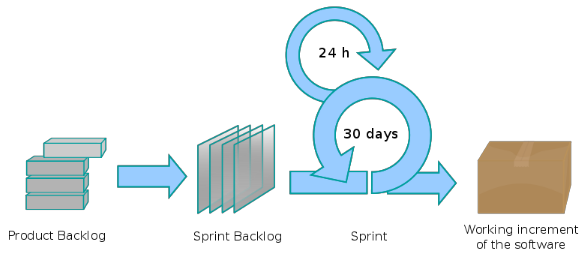
\includegraphics[scale=0.4]{images/scrum_process.png}
\caption{Scrum process}
\end{figure}

\paragraph{Documents}
\begin{itemize}
\item Product backlog: List of \emph{ordered} requirements for the product;
\item Sprint backlog: Requirements or activities for the sprint;
\item Increment: All what is done in all sprints. It must be usable.
\end{itemize}

\paragraph{Meetings}
\begin{itemize}
\item Daily scrum: Stand-up, 15 minutes;
\item Sprint planning meeting: One day;
\item Sprint reviewing meeting: Presentation to customer (demo), 4 hours;
\item Sprint retrospective (post mortem): Introspective.
\end{itemize}

\begin{table}
\centering
\small
\begin{tabularx}{0.95\textwidth}{X|X|X|X}
& \textbf{Waterfall} & \textbf{RUP} & \textbf{Agile} \\
\hline
\textbf{Activities} & Sequential & Parallel & Parallel \\
\hline
\textbf{Iterations} & One, long & One, long with sub iterations & Many, short \\
\hline
\textbf{Emphasis on documents} & Heavy & Mild & No \\
\end{tabularx}
\caption{Options}

\begin{tabularx}{0.95\textwidth}{X|X|X|X}
& \textbf{Waterfall} & \textbf{RUP} & \textbf{Agile} \\
\hline
\textbf{New development / Maintenance} & Mostly new development & Mostly new development & Both \\
\hline
\textbf{Compliance} & Yes & Partial & No \\
\hline
\textbf{Size} & Large projects, distributed teams and contractors & Also large projects, distributed teams & Small projects, co-located teams \\
\end{tabularx}
\caption{Suitability}
\end{table}

\subsection{eXtreme Programming}
The fundamental idea behind \emph{eXtreme Programming} is to have very short iterations with fast deliveries, by performing continuous testing and exploiting pair programming. eXtreme Programming is based on some basic facts:
\begin{itemize}
\item Producing code is required to deliver a system;
\item Money spent on analysis and design are wasted if the system is never used;
\item Business requirements have to be the drivers for software development;
\item Requirements change.
\end{itemize}
and requires four values:
\begin{itemize}
\item Communication: face to face, rather than document driven;
\item Simplicity: build a simple thing that should work;
\item Feedback: put system into production as soon as possible;
\item Courage: at every iteration it is possible to change many misunderstood or useless things.
\end{itemize}

\subsubsection{Practises}
\paragraph{On-site customer}
Real customer has to be part of the team, in order to define business needs, answer questions, resolve issues and prioritize features.

\paragraph{Small releases}
Put system into production as soon as possible in order to receive a fast feedback, delivering valuable features first in short cycle time, because planning 1-2 months is easier than planning 6-12 months.

\paragraph{Metaphor/Architecture}
Long documents may not be read by all people. Therefore, it is better to have a short description, i.e.,\@ metaphor, including few concepts which can be well understood, shared and agreed by all the people involved. Therefore, the initial architecture is actually a prototype of the final architecture.

\paragraph{Simple design}
The ``right'' design will run all tests, fulfills all current business requirements avoiding code duplication and using fewest possible classes and methods, remembering that design is made for today, not for the future.

\paragraph{Refactoring}
\emph{Refactoring} consists of restructuring the system without changing the functionality with the goal of keeping design simple, e.g.,\@ by changing bad design if found or removing dead code. Refactoring is useful to improve some non functional properties, e.g.,\@ maintainability, usability, performance by changing internal design.

From a business point of view, this is a useless procedure because, actually, it does not produce any delivery (functionality)

\paragraph{Pair programming}
All production code is written with two people looking at one machine and pairs change all the time. In this way, code is permanently inspected but it is possible that some development time is needed.

With respect to solo programming, quality should increase, duration should decrease and effort should increase, i.e.,\@ Pair programming favors quality, reduces duration and increases effort. Effect of group dynamics and skill of pairs must be considered, some guidelines are shown in table~\ref{tab:pp_guidelines}.

\begin{table}
\centering
\small
\begin{tabularx}{0.95 \textwidth}{|l|l|X|}
\hline
\textbf{Experience} & \textbf{Task complexity} & \textbf{Use of pair programming} \\
\hline
Junior & Easy & Yes, provided that increased quality is the main goal. \\
\cline{2-3}
 & Complex & Yes, provided that increased quality is the main goal. \\
\hline
Intermediate & Easy & No. \\
\cline{2-3}
 & Complex & Yes, provided that increased quality is the main goal. \\
\hline
Senior & Easy & No. \\
\cline{2-3}
 & Complex & No, unless you are sure that the task is too complex to be solved satisfactorily by an individual senior programmer. \\
\hline
\end{tabularx}
\caption{Guidelines for when to use pair programming}
\label{tab:pp_guidelines}
\end{table}

\paragraph{Test driven development}
Automatic test drivers. Test are written before code production from developers and customers, with a strong emphasis on regression testing in such a way that unit tests pass 100\% and the code is always under testing.

\paragraph{Planning game}
\begin{itemize}
\item Business decisions:
\begin{itemize}
\item Which ``stories'' should be developed;
\item Priority of stories;
\item Composition of releases;
\item Release dates. 
\end{itemize}
\item Technical decisions:
\begin{itemize}
\item Time estimates for features/stories;
\item Elaborate consequences of business decisions;
\item Team organization and process;
\item Scheduling.
\end{itemize}
\end{itemize}

\paragraph{Sustainable development}
Developing full speed only works with fresh people. Working overtime for two weeks in a row indicates problems.

\paragraph{Collective ownership}
All code can be changed by anybody on the team and everybody is required to improve any portion of bad code he/she sees. Individual code ownership tends to create experts.

\paragraph{Contiguous integration}
Integration happens after a few hours of development.Code is released into current baseline on integration machine and all test are run, possibly during the night or when the system is not ``stressed''. In case of errors, the previous version is restored and problems are fixed before the next release.

\paragraph{Coding standards}
In order to achieve collective ownership, teams has to adopt a coding standard which makes other people's code more understandable and avoids code changes because of syntactic preferences.

\paragraph{Environment}
The \emph{environment} has to support communication among developers, e.g.,\@ open space or common spaces. It is evident that the working environment has great influence on quality and quantity of work. Interruptions by colleagues, email or meetings and lack of comfort due to noise or light are negative factors.

\section{Maintenance process}
Change is the key element in a \emph{maintenance} process. A change can be
\begin{itemize}
\item A defect to be fixed (corrective maintenance); \item A modification to an existing function (perspective maintenance);
\item A new function (evolutive maintenance).
\end{itemize}
Changes can be originated by end users or developers and are received and processed by a group of maintainers.

The product evolves by applying a flow of changes, typically with regular releases which can be major, i.e.,\@ every few months, or minor/critical, i.e.,\@ when needed. The stable baseline is released regularly, while the working baseline is the one where maintainers work.

\paragraph{Process}
\begin{enumerate}
\item Receive change request;
\item Filter:
\begin{itemize}
\item Merge similar change requests;
\item Discard unfeasible or incorrect change requests;
\end{itemize}
\item Assess:
\begin{itemize}
\item Evaluate impact of change request in terms of effort/cost, feasibility, impact on architecture and/or functionality;
\item Rank change requests, using severity for the corrective ones and importance for the evolution ones;
\end{itemize}
\item Assign change request to a (team of) maintainer;
\item Implement change request
\begin{itemize}
\item Design, code, unit test, integration test;
\item System test;
\item Insert in next release.
\end{itemize}
\end{enumerate}
Only a part of change requests, even corrective, are actually implemented.

The flow of changes can radically change a product over time, therefore it is needed to control or maintain architecture in order to prevent architecture erosion and it is needed to control suitability for market and users.

\begin{figure}[hbtp]
\centering
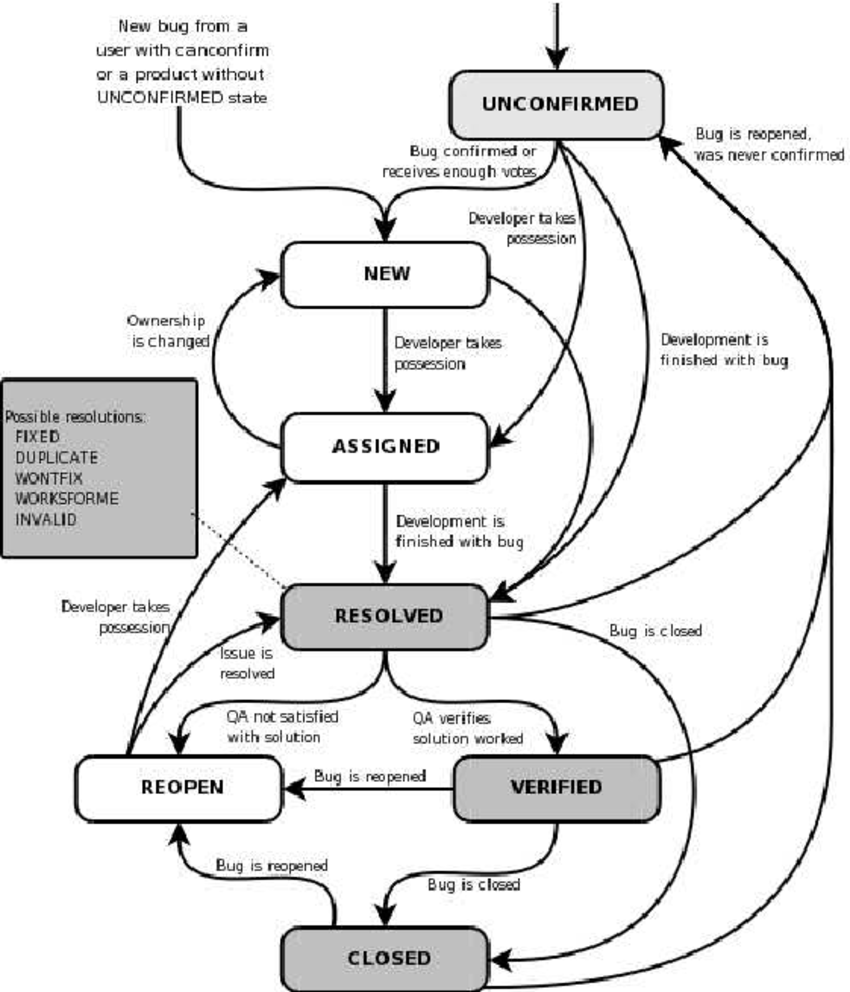
\includegraphics[scale=0.35]{images/bug_lifecycle.png}
\caption{Lifecycle for change (bug)}
\end{figure}

\section{Real cases}
\subsection{Ferrari}
\paragraph{Products}
\begin{itemize}
\item Electronic Control Unit ECU (embedded software):
\begin{itemize}
\item Power unit: engine, energy recovery;
\item Gearbox;
\item Brakes.
\end{itemize}
\item Support tools:
\begin{itemize}
\item Simulation of car;
\item Telemetry;
\item Configuration;
\item Pit stop control.
\end{itemize}
\end{itemize}

\paragraph{Process and toolchain}
\begin{enumerate}
\item Simulink model;
\item Translation to C;
\item Compilation to assembly;
\item Configuration and tuning;
\item Upload to firmware.
\end{enumerate}

\paragraph{Process and timing}
About two weeks between races:
\begin{itemize}
\item Requirements: 2 days;
\item Coding: 2 days;
\item Test: 4 days;
\item FIA freezing: 3 days;
\item Race: 3 days.
\end{itemize}
In one season, from March to November:
\begin{itemize}
\item 300 versions of embedded code;
\item 100 versions tools;
\item 1000 change requests, including few trivial bugs and tens of conceptual defects, i.e.,\@ requirement misunderstandings).
\end{itemize}
Issues are due to tight schedule and interaction among mechanical and software engineers.

\subsection{Apache}
\paragraph{Process}
Process is organized as an evolution/maintenance process spanning many years.
\begin{itemize}
\item Tools:
\begin{itemize}
\item CVS;
\item Mailing list;
\item Bugzilla (bug tracking).
\end{itemize}
\item Products:
\begin{itemize}
\item Source code;
\item Test cases;
\item Informal documentation (mails, bugs, comments).
\end{itemize}
\end{itemize}

\paragraph{Roles}
\begin{itemize}
\item Core team (2-8 people);
\item Patch developers (10-100 people);
\item Bug providers (100-1000+ people);
\item Others.
\end{itemize}

\paragraph{Facts}
\begin{itemize}
\item Limited documentation:
\begin{itemize}
\item No project plan, no quality plan, no requirement document.
\end{itemize}
\item Key points:
\begin{itemize}
\item Strict CVS;
\item Simple and effective tools for bug and change tracking;
\item Hierarchy of roles and responsibilities;
\item Motivated developers, especially in core team.
\end{itemize}
\end{itemize}

\subsection{Synchronize and Stabilize}
This approach was adopted by Microsoft from 1993 to 1995. It is a variant of the RUP and it is applicable in contexts where requirements can be fixed early on and it is needed to build complex products (millions of line of codes) with several interacting components, therefore with a design hard to devise and freeze early on.

\paragraph{Planning phase}
\begin{itemize}
\item Vision statement - Product managers:
\begin{itemize}
\item Define goals for the new products;
\item Priority order user activities that need to be supported by product features.
\end{itemize}
\item Deliverables:
\begin{itemize}
\item Specification document;
\item Schedule and ``feature team'' information:
\begin{itemize}
\item 1 program manager;
\item 3-8 developers;
\item 3-8 testers (1:1 ratio with developers\footnote{The idea is to spend half of the time for testing.}).
\end{itemize}
\end{itemize}
\end{itemize}

\paragraph{Development phase}
\begin{itemize}
\item Plan 3-4 subprojects (iterations) lasting 2-4 months each;
\item Buffer time between iterations;
\item Subprojects require design, code and debug, starting from the most critical features and shared components.
\end{itemize}

\subparagraph{Subproject development}
Feature teams go through the complete development cycle, feature integration, testing and fixing problems, synchronizing work by building the product, finding and fixing errors on a daily and weekly basis. Testers are paired with developers.

\paragraph{Stabilization phase}
\emph{Stabilization} requires testing (internal and/or external) and release preparation.

\subsection{Cyber physical ecosystems}
This approach is adopted by Wikipedia, Google, Twitter and in all products where a ``city model'' can be adopted:
\begin{itemize}
\item No clear boundary (APIs and mash ups);
\item Requirements are never known and emerge from individual contributions;
\item Continuous evolution without any release or planning;
\item Continuous operation without clear development and maintenance phases, always on and always changing;
\item Always ``beta'';
\item Emergent behaviors.
\end{itemize}

\paragraph{Structure}
\begin{itemize}
\item Core/Kernel providing horizontal functions: always on, top reliability, closed and slow to change. Requirements and architecture are well defined, controlled by core team; 
\item Periphery providing end user functions and content: fast changing, open. Requirements and design are unclear, unstable and crowdsourced without control.
\end{itemize}

\section{Process selection}
\paragraph{Process attributes}
\begin{itemize}
\item Sequential or parallel activities;
\item Iterations or no iterations;
\item Time framed or not;
\item Colocation of staff;
\item Emphasis on documents.
\end{itemize}

\begin{table}
\centering
\begin{tabular}{|l|l|l|l|l|}
\hline
& \textbf{Agile} & \textbf{26262} & \textbf{RUP} & \textbf{Sync Stab} \\
\hline
\textbf{Iteration number} & Many & One+ & Few & Few \\
\hline
\textbf{Iteration duration} & Weeks & Long & Months & Months \\
\hline
\textbf{Parallel activities} & Yes & No & Yes & Yes \\
\hline
\textbf{Documents} & Few & Many & Many & Few \\
\hline
\textbf{Colocation staff} & Yes & Yes or not & \multicolumn{1}{c|}{-} & Yes \\
\hline
\end{tabular}
\caption{Process comparison}
\end{table}

\subsection{Product attributes}
\paragraph{Criticality}
\emph{Criticality} defines emphasis on reliability, safety and security. Norms and laws may be applied, about legal responsibilities, too.

\paragraph{Size}
\emph{Size} can be evaluated in line of codes, in duration of development and team size or number of subcontractors. Size affects coordination and communication during development and maintenance.

\paragraph{Domain}
\emph{Domain} has effect on norms and laws applied, e.g.,\@ Basel~3 in finance, 26262 in automotive, and responsibility of developer, operator and maintainer.

\paragraph{Lifecycle}
Expected \emph{lifecycle} has effects on tradeoff development cost vs maintenance cost. Each lifecycle phase can be either a new development or a maintenance activity.

\paragraph{Bespoke or Market driven}
It has effect on time to market, requirement collection and ranking, cost structure and business model.
\begin{itemize}
\item Bespoke: one customer or end user;
\item Market driven: Many customers or end users.
\end{itemize}

\paragraph{Ownership}
\emph{Ownership} has effect on capability of modifying code, i.e.,\@ parametrization or adaptation. It can be full property, copyright, copyleft.

\paragraph{Relationship with developer}
\emph{Developer} can be the same as end user, an internal department of the company or an external company.

\subsection{Rules of thumb}
\begin{itemize}
\item Reliability, safety: waterfall-like (document based, few iterations, no parallel activities);
\item Market driven (time to market): frequent iterations;
\item Colocation of staff: if no, document-based and no parallel activities;
\item Size: the bigger, the more documents and activities;
\item Lifetime: if long, documents are required.
\end{itemize}